\documentclass[crop,tikz]{standalone}% 'crop' is the default for v1.0, before it was 'preview'
\usepackage{pgfplots}
\usetikzlibrary{math}
\begin{document}
    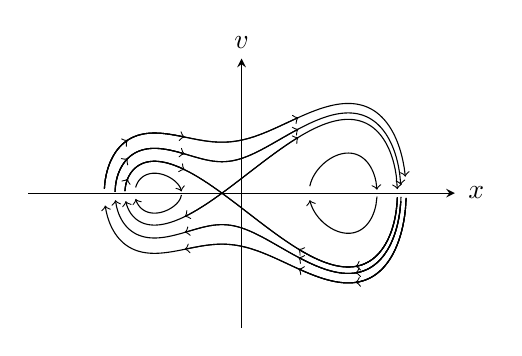
\begin{tikzpicture}
  	\tikzmath{\xa = 2; \y = 3; \lim = 1.6;}
	\begin{axis}[
	    width=7cm,
	    height=5cm,
	    xmin= -\xa, xmax= \xa,
	    ymin= -\y, ymax = \y,
	    axis lines = middle,
	    x label style={at={(axis description cs:1.05,0.56)},anchor=north},
	    y label style={at={(axis description cs:0.5,1)},anchor=south},
	    xlabel={$x$},
	    ylabel={$v$},
	    xtick={0},
	    xticklabels={$0$},
	    ytick={0},
	    yticklabel={},
	    ]
	    \foreach \s in {0,1,2, 2.5} { % Traccio più linee per avere più punte di freccia
		\foreach \E in {1.354 , 1.6, 2} { % Vario l'energia per vedere le tre aree dello spazio delle fasi
		    %%%%%%%%%%%%%%%%%%%%%%%%%%%%%%%%%%%%%%%%%%%%%
		    %  Linee del moto al variare della energia  %
		    %%%%%%%%%%%%%%%%%%%%%%%%%%%%%%%%%%%%%%%%%%%%%
		    %((x+1)^2+0.5)*(x-1)^2
		    %(-x^2/2*(1-x^2/2) + 0.3)
		    \addplot [domain= ( -\lim): ( \lim) - 2*\lim*\s/3, samples=300, ->] {sqrt( 2*(\E - ((x+1)^2+0.3)*(x-1)^2)  )};
		    \addplot [domain= ( -\lim) + 2*\lim*\s/3: ( \lim) , samples=300, <-] {-sqrt( 2*(\E - ((x+1)^2+0.3)*(x-1)^2) )};
		}
	    }
	    \addplot [domain= ( 0): ( 1.9), samples=200, ->] {sqrt( 2*(0.4 - ((x+1)^2+0.3)*(x-1)^2)  )};
	    \addplot [domain= ( 0): ( 1.9) , samples=200, <-] {-sqrt( 2*(0.4 - ((x+1)^2+0.3)*(x-1)^2) )};
	    \addplot [domain= ( -1.9): ( 0), samples=200, ->] {sqrt( 2*(1.2 - ((x+1)^2+0.3)*(x-1)^2)  )};
	    \addplot [domain= ( -1.9): ( 0) , samples=200, <-] {-sqrt( 2*(1.2 - ((x+1)^2+0.3)*(x-1)^2) )};
	\end{axis}
    \end{tikzpicture}
\end{document}
